% !TEX root = ../master-thesis.tex

The ability to prepare arbitrary atom configurations is a key ingredient for bottom-up quantum simulation. After obtaining unit filling for both spin states (as discussed in Sec.~\ref{subsec:balancing} and \ref{subsec:spin-selective-spilling}), we implement a multi-stage spilling sequence that enables spin- and site-resolved initialization of arbitrary patterns.

The loading sequence proceeds in several steps:
\begin{enumerate*}
    \item Prepare a $\ket{1}$–$\ket{2}$ spin mixture with unit filling across the tweezer array.
    \item Perform global spilling steps to remove atoms from factorized intensity patterns $P_{ij}$, affecting both spin states.
    \item Apply spin-selective spilling steps to remove atoms in state $\ket{1}$ from additional factorized subsets of sites.
    \item Flip the remaining atoms $\ket{1} \leftrightarrow \ket{2}$ using a microwave $\pi$-pulse.
    \item Repeat spin-selective spilling to further refine the configuration
\end{enumerate*}

% \textbf{Factorized removal.}
Each spilling step removes atoms from sites where the local tweezer depth $P_{ij}$ falls below a certain threshold. Since we can impose any rank-1 intensity mask $P_{ij} = H_i V_j$, it is possible to tailor the removal region to arbitrary product forms. To remove a single atom at site $(i', j')$, for example, we reduce $H_{i'}$ and $V_{j'}$ by a factor $\eta < 1$ and simultaneously increase the global power by $\eta$. This yields a relative intensity of $1/\eta$ at the intersection, while leaving all other sites unchanged or increased in depth. In this way, we can reliably isolate and remove atoms from any desired factorized subset.

% \textbf{Boolean decomposition.}
We represent the cumulative removal pattern as a binary matrix $W_{ij}$, where $W_{ij} = 1$ indicates that the atom at site $(i, j)$ has been removed. Each spilling operation adds a binary outer product $u^\lambda_i v^\lambda_j$ via Boolean logic ($1 + 1 = 1$). An arbitrary target pattern can therefore be reached through a sequence of such operations:
\begin{equation}
    \label{eq:ebmf}
    W_{ij} = \bigvee_{\lambda=1}^{r} u^\lambda_i v^\lambda_j,
\end{equation}
which defines the exact Boolean matrix factorization (EBMF) of the removal matrix. In the worst case, any binary $n \times n$ matrix admits such a decomposition using at most $n$ steps.

% \textbf{Optimal EBMF.}
While a naive strategy—such as row- or column-wise removal—may require up to $n$ iterations, we find that optimal EBMF often reduces this number. The problem of finding an exact Boolean matrix factorization with minimal rank is known to be NP-complete~\cite{orlin_contentment_1977} and NP-hard to approximate~\cite{gruber_inapproximability_2007}. Nevertheless, for arrays up to $10 \times 10$, optimal decompositions can be computed in a few seconds using a SAT solver. These improvements are particularly useful for minimizing experimental cycle time and improving overall sequence fidelity. A full discussion of the EBMF algorithm and its implementation is presented in Appendix.



\begin{figure}
    \centering
    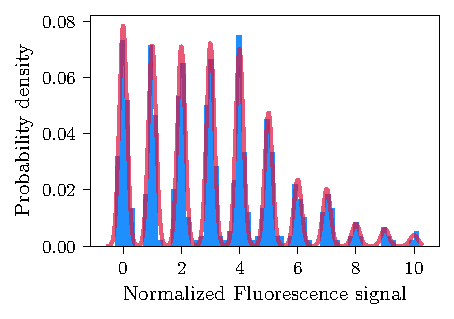
\includegraphics{fig-py/atom-counting.pdf}
    \caption[Single atom counting]{
        \textbf{Single atom counting.}
        Calibration histogram for single-atom counting based on fluorescence signal after after loading to the MOT. Clear quantized peaks correspond to integer atom numbers; the solid red line is a multi-Gaussian fit to the distribution. 
    }
    \label{fig:spillingadd}
\end{figure}